\section{Wie kann der Begriff Kraftwerksreserve definiert werden?}

	Da der Begriff Kraftwerksreserve nicht genau definiert ist, wird im Folgenden auf die unterschiedlichen Arten der Kraftwerksreserven eingegangen.
	Grundlage bildet der Strommarkt, welcher in Kapitel \ref{sect: Wie funktioniert der deutsche Strommarkt?} behandelt wird.
	Aufgrund der Folgen des Ukraine-Konflikts ist ebenfalls eine weitere Art der Reserve hinzugekommen.

	\subsection{Wie funktioniert der deutsche Strommarkt?} \label{sect: Wie funktioniert der deutsche Strommarkt?}
	
		In Deutschland gibt es einen Energy-Only-Market (EOM).
		Dies bedeutet, dass ausschließlich der tatsächlich produzierte Strom gehandelt wird.
		Anders wäre dies bei dem viel diskutierten Kapazitätsmarkt, indem auch vorgehaltene Leistungen für z.B. Dunkelflauten vergütet werden (haucap).
		Die Preisbildung folgt dem Prinzip der Merit-Order (s. Abb. \ref{Abb. Strompreisbildung Merit Order}).
		In der Merit-Order werden alle Stromproduzenten, welche zu gegebenen Zeitpunkt ihren Strom am Markt anbieten, nach ihren jeweiligen Grenzkosten aufsteigend aufgelistet.
		Der Stromerzeuger mit den geringsten Grenzkosten, darf als erstes einspeisen und nach ihm derjenige mit den nächst größeren Grenzkosten.
		Als Grenzkosten werden die Erzeugungskosten für die auf dem Markt genau angebotene Strommenge bezeichnet.
		Der Stromproduzent, welcher mit seiner angebotenen Strommenge Angebot und Nachfrage deckt, legt den zu vergütenden Strompreis für alle anderen Marktteilnehmer in der Merit-Order unter ihm fest.
		Dieses Kraftwerk heißt Grenzkostenkraftwerk.
		In Abbildung \ref{Abb. Strompreisbildung Merit Order} ist die Reihenfolge der Stromerzeugungsart und den typisch zu erwartenden Grenzkosten dargestellt. \\
		
		\begin{figure} [H]
			\centering
			\label{Abb. Strompreisbildung Merit Order}
			\includegraphics[page=82,trim=150 282 140 375, clip, width=0.85\textwidth]{./anhang/Doktorarbeit Reitsam.pdf}
			\caption{Strompreisbildung an der Börse nach dem Merit-Order-Prinzip \parencite{Doktorarbeit_Reitsam}}
		\end{figure}
		
		In der Merit-Order weist die Stromerzeugung aus erneuerbaren Energien Grenzkosten von nahezu Null auf.
		Die Folge des Ausbaus von erneuerbaren Energien ist, dass konventionelle Kraftwerke mit hohen Grenzkosten, vor allem Gas- und Ölkraftwerke, in der Reihenfolge nach rechts gerückt werden (Merit-Order-Effekt, s. Abb. \ref{Abb. Strompreisbildung Merit Order}).
		Das Verdrängen der Gas-,Öl- sowie Pumpspeicherkraftwerke führen zu einem sinkenden Strompreis an der Böse \parencite{Frauenhofer_PV_Bericht}.
		Dadurch sind diese Kraftwerke nur bei mangelndem Wind und mangelnder Sonneneinstrahlung an der Stromproduktion beteiligt.
		Für den Strompreis bedeutet dies teilweise erhebliche Schwankungen je nach aktueller Wetterlage und geringe bzw. unvorhersehbare Betriebsstunden der genannten Marktteilnehmer. 
		Damit werden die Anreize vor allem schnell regelbare Gaskraftwerke zu errichten und wirtschaftlich betreiben zu können deutlich eingedämmt, weil die Kraftwerksleistung ohne Vergütung vorgehalten wird \parencite{Frauenhofer_PV_Bericht}.
		Gegensätzlich dazu verlangt der Ausbau regenerativer Stromerzeuger einen Zuwachs schnell regelbarer Gaskraftwerke, um plötzlich auftretende Schwankungen auszugleichen \parencite{Doktorarbeit_Reitsam}. \\
		
		Die Forderung eines Kapazitätsmarkts, indem auch vorgehaltene Kraftwerksleistung bepreist wird, gewinnt dahingehend an Bedeutung.
		Den Karftwerksbetriebern fällt es zunehmend schwer ihre konventionellen Kraftwerke aufgrund der bereits erörterten fehlenden und unvorhersehbaren Betriebsstunden rentabel zu betreiben.
		Auch ohne weiteren Ausbau von erneuerbaren Energien wird bei Dunkelflauten gerade in den wenig sonnigen Wintermonaten Januar und Februar weiterhin Residuallast gebraucht.
		Konträr dazu wurde eine strategische Kraftwerksreserve aus Braunkohlekraftwerken aufgebaut \parencite{bbh_blog}.		
				
	\subsection{Kraftwerksreserven zur Netzfrequenzstabilisierung}
	
		\begin{wrapfigure}{r}{0.55\textwidth}
			\centering
			\includegraphics[page=92,trim=260 71 50 450, clip, width=0.4\textwidth]{./anhang/Elektrizitätswirtschaft.pdf}
			\caption{Regelzonen und Übertragungsnetzbetreiber in Deutschland \parencite{Elektrizitätswirtschaft}}
			\label{Abb. Regelzonen Deutschland}
		\end{wrapfigure}
	
		Die Kraftwerksreserven zur Netzfrequenzstabilisierung fallen unter den Begriff des Regelenergiemarkts.
		Aufgrund des liberalisierten Strommarkts besitzen die Übertragungsnetzbetreiber keine eigenen Kraftwerke, sodass für die Stabilisierung Verträge mit Energieversorgungsunternehmen (EVU) geschlossen werden müssen. \\
			
		Unter Regelenergie versteht man zum einen die Reservierung von Kraftwerksreserven bzw. -kapazitäten (Regelleistung) und zum anderen den Ausgleich von Regelzonenungleichgewichten (Regelarbeit) \parencite{Elektrizitätswirtschaft}.
		Da es im Stromnetz zu negativen und positiven Abweichungen der Frequenz kommen kann, wird zur Kompensation sowohl positive als auch negative Regelarbeit benötigt.
		Anders als bei der Regelleistung wird eine gelieferte Strommenge in \si{\mega\watt\hour} vergütet.
		Um Unterschiede zwischen Angebot und Nachfrage unter den vier deutschen Regelzonen zu decken, wird eine Reservierung von Kraftwerksreserven erforderlich (Regelzonen s. Abb. \ref{Abb. Regelzonen Deutschland}). 
		In diesem Fall erfolgt eine Bezahlung der Kraftwerke unabhängig von der gelieferten Strommenge und Einsatzzeit \parencite{Elektrizitätswirtschaft}. 
		Die Bezahlung ist als eine Art Entschädigung für das Vorhalten von Kraftwerkskapazitäten, gegebenenfalls nicht Abrufen und den damit verbundenen Fixkosten der Einsatzbereitschaft zu verstehen.   
		
		\begin{figure} [H]
			\centering
			\label{Abb. Beispielhafte Darstellung der Regelenergie in Abhängigkeit der Netzfrequenz}
			\includegraphics[page=115,trim=50 80 50 470, clip, width=\textwidth]{./anhang/Elektrizitätswirtschaft.pdf}
			\caption{Beispielhafte Darstellung der Regelarbeit in Abhängigkeit der Netzfrequenz \parencite{Elektrizitätswirtschaft}}
		\end{figure}
	
		Um die Frequenz von \SI{50}{\hertz} im deutschen und europäischen Stromnetz stabil zu halten, muss ständig Regelarbeit eingesetzt werden.
		Für das ständige Abrufen der Regelarbeit wird Regelleistung gebraucht.
		Für die Netzfrequenz gibt es eine zulässige Schwankungsbreite von $\pm\SI{10}{\milli\hertz}$ \parencite{Angerer_Krohns}.
		Erst ab Unterschreitung von \SI{49,99}{\hertz} bzw. Überschreitung von \SI{50,01}{\hertz} wird die Frequenz durch Einsatz von Regelenergie stabilisiert.
		Bei einer zu geringen Netzfrequenz ist zu wenig Strom im Netz aufgrund von zu großer Abnahme oder Produktionsausfällen seitens der Stromerzeuger.
		In diesem Zuge gibt es Marktteilnehmer, welche zusätzliche Reserven bzw. Kapazitäten anbieten oder Stromverbraucher, die ihren eigenen Verbrauch drosseln.
		Gegensätzlich dazu ist eine zu hohe Netzfrequenz auf zu viel Strom im Netz zurückzuführen. 
		In diesem Fall wiederum können Stromverbraucher diesen erhöhen oder Stromerzeuger ihre Kraftwerksleistung herunterfahren. 
		In Abbildung \ref{Abb. Beispielhafte Darstellung der Regelenergie in Abhängigkeit der Netzfrequenz} ist die Abhängigkeit der Regelarbeit von der Netzfrequenz dargestellt.
		Für die beschrieben Mechanismen gibt es im Wesentlichen drei Regelenergien, die Primär-, Sekundärregelenergie und die Minutenreserve.
		Die Abbildung \ref{Abb. Reaktionskette Regelenergien} zeigt Regelenergiearten in ihrer Einsatzreihenfolge und Reaktionsschnelligkeit zur Stabilisierung der Netzfrequenz. 
		
		\begin{figure} [H]
			\centering
			\label{Abb. Reaktionskette Regelenergien}
			
\includegraphics[page=209,trim=40 465 40 205, clip, width=\textwidth]{./anhang/Monitoringbericht_Energie2021.pdf}
			\caption{Zeitliche Abfolge der Regelleistungsreserven zur Netzfrequenzstabilisierung \parencite{Elektrizitätswirtschaft}}
		\end{figure}
		
		\subsubsection{Primärregelreserve} \label{sect: Primärregelreserve}
		
			Der Eingriff durch die Primärregelreserve (PRL) erfolgt unmittelbar nach Über- sowie Unterschreitung des zulässigen Frequenzbereichs durch die Anbieter von Primärreserven.
			Die Bereitstellung erfolgt über das Gebiet der ENTSO-E ("`European Network of Transmission System Operators for Electricity"').
			Da es sich bei dem ENTSO-E um ein Synchrongebiet mit \SI{50}{\hertz} Netzfrequenz handelt, wird die Bereitstellung von Primärregelleistung unter allen Teilnehmern, gemessen am eingespeisten Strom, aufgeteilt.
			Die Mitglieder können der Abbildung \ref{Abb. Mitglieder ENTSO-E} entnommen werden.
			Die gesamte Kapazität aller Mitglieder beläuft sich auf $\pm\SI{3}{\giga\watt}$ und wird anhand des zeitgleichen Ausfalls der zwei größten Kraftwerksblöcke innerhalb des Verbundnetzes ermittelt.
			Am Ort des Anbieters wird die Netzfrequenz gemessen, um schnell und frequenzabhängig Strom einzuspeisen oder zu speichern. 
			Innerhalb von \SI{30}{\second} muss die komplette Regelleistung abrufbar sein und die vollständig angebotene Regelarbeit für \SI{15}{\minute} geliefert werden.
			Der Regelbereich befindet sich dabei innerhalb des Regelbands und außerhalb des Totbands (s. Abb. \ref{Abb. Regelung Primarregelleistung} next Kraftwerke).
			Ab einer Netzfrequenz von \SI{49,99}{\hertz} bzw. \SI{50,01}{\hertz} muss der Stromlieferant die Primärregelleistung hochfahren und bei einer Frequenz von \SI{49,8}{\hertz} bzw. \SI{50,2}{\hertz} \SI{100}{\percent} seiner angebotenen Leistung abrufen bzw. liefern können. 
			
			\begin{figure}[H]
				\centering
				\includegraphics[page=1,trim=70 70 70 120, clip, width=0.6\textwidth]{./anhang/frc-map.png}
				\caption{Mitglieder der ENTSO-E für PRL\parencite{ENTSO-E_PRL}}
				\label{Abb. Mitglieder ENTSO-E}
			\end{figure}
			
			Die Ausschreibung von Primärregelleistung erfolgt täglich für einen Erbringungszeitraum vom Folgetag 0:00 Uhr bis 24:00 Uhr.
			Angebotsabgabe erfolgt am Vortag bis 8:00 Uhr  \parencite{regelleistungnet_PRL_Ausschreibung}.
			Die Auktion erfolgt online über die Internetseite regelleistung.net \parencite{regelleistungnet_PRL_Ausschreibung}.
			Zuschlag bekommen diejenigen Anbieter, welche für den ÜNB am wirtschaftlichsten sind.
			Der Anbieter, welcher Angebot und Nachfrage deckt, legt den Leistungspreis für alle anderen Zuschläger fest ("`Marginal Pricing"').
			In Tabelle \ref{Tab. Merkmale der Primärregellung} sind die wichtigsten Eckpunkte der Primärregeleistung dargestellt.		
		
			\begin{table}[H]
				\centering
				\caption{Merkmale der Primärregelleistung \cite{Regelleistung_NextKraftwerke}}
				\label{Tab. Merkmale der Primärregellung}
				\begin{tabular}{ll}
					\hline
					Regelenergieart & Primärregelleistung  \\ \hline
					Bereitstellung durch & ENTSO-E  \\
					Aktivierung & \makecell[l]{Frequenzgesteuert: \\ Eigenständige Messung/Eingriff vor \\ Ort durch Anbieter der PRL} \\
					Volle Leistung & Innerhalb von 30 Sekunden \\
					\makecell[l]{Abzudeckender Zeitraum \\ nach Störungsfall} & \num{0} bis \num{15} Minuten  \\
					Vergütung & Leistungspreis  \\
					Mindestangebots-größe & Ab $\pm\SI{1}{\mega\watt}$ (symmetrisch) \\
					Tägliche Produkte & \makecell[l]{Positiv und negativ: \\ \num{6} Zeitintervalle über \num{4} Stunden} \\ \hline
				\end{tabular}
			\end{table}
		
		\subsubsection{Sekundärregelreserve}		
			
			Bei länger anhaltender Frequenzabweichung wird die Sekundärregelreserve (SRL) hinzu geschaltet, um die Frequenz durch sowohl positive als auch negative Regelleistung wieder zu stabilisieren.
			Sie wird durch den innerhalb der Regelzone aktiven Übertragungsnetzbetreiber per Signal angefordert und durch die an der Auktion teilgenommenen Anbieter von SRL abgerufen. 
			Die SRL wird nach \num{30} Sekunden hinzu geschaltet und muss nach fünf Minuten volle Regelarbeit liefern können. 
			Für den täglichen Abruf der Reserve gibt es sechs Zeitscheiben mit je vier Stunden.
			Aufgrund dessen, dass die Sekundärregelleistungsanbieter ihre Anlagen im Verbund nicht auf einige \si{\mega\watt} modulieren können, besteht kontinuierlicher Bedarf an Sekundärregelleistung.
			Da jeder ÜNB in seiner Regelzone SRL zu- und abschalten kann, besteht eine Austauschpflicht unter den vier ÜNB.
			Der Grund ist, dass auf diese Weise ineffizientes gegeneinander regeln vermieden werden soll \parencite{SRL_NextKraftwerke}. \\
			
			Die Mindestangebotsgröße beträgt \SI{5}{\mega\watt} und nach einer Änderung des Beschlusses "`zur Festlegung von Ausschreibungsbedingungen und Veröffentlichungspflichten für Sekundärregelung"' der BNetzA können auch Angebote in Höhe von \SI{1}{\mega\watt} bis \SI{4}{\mega\watt} eingereicht werden.
			Diese Änderung ist an die Maßgabe geknüpft, dass die Anbieter ausschließlich ein Angebot je Produktscheibe für positive oder negative Regelleistung abgeben dürfen \parencite{Beschluss_SRL}.
			Die Reduzierung erleichtert den Eintritt für kleinere Anbieter oder jene, welche mehrere Anlagen poolen und meist zu virtuellen Kraftwerken verbinden. \\
			
			Die Ausschreibungen für die Sekundärregelreserven finden täglich statt. 
			Bis zum Vortag um 9:00 Uhr muss das Angebot für den Folgetag abgegeben werden.
			Es wird aufgeteilt nach dem Leistungs- und Arbeitspreis vergütet.
			Dies bedeutet, dass jeder Anbieter einen Festpreis für die Vorhaltung der angebotenen Leistung abgibt, egal ob diese abgerufen wird (Handel auf dem Regelleistungsmarkt).
			Der abgegebene Arbeitspreis wird auf dem Regelarbeitsmarkt gehandelt und gibt an wie hoch die Vergütung je erbrachter \si{\mega\watt\hour} ist.
			Die Art der Vergabe erfolgt nach der aufgestellten Merit-Order-Liste allerdings in einem Pay-as-Bid Verfahren(s. Kapitel \ref{sect: Primärregelreserve}).
			Es wird lediglich der angebotene Preis vergütet und nicht wie bei der PRL durch das "`Marginal Pricing"'.
			Tabelle \ref{Tab. Merkmale der Sekundärregelreserve} zeigt nochmals die wichtigsten Eckdaten der Sekundärregelreserve.
			
			\begin{table}[H]
				\centering
				\caption{Merkmale der Sekundärregelreserve \cite{Regelleistung_NextKraftwerke}}
				\label{Tab. Merkmale der Sekundärregelreserve}
				\begin{tabular}{ll}
					\hline
					Regelenergieart &  Sekundärregelreserve  \\ \hline
					Bereitstellung durch  & ÜNB  \\
					Aktivierung & \makecell[l]{Durch verantwortlichen ÜNB \\ - manuelle Anforderung durch ÜNB} \\
					Volle Leistung & Innerhalb von 5 Minuten \\
					\makecell[l]{Abzudeckender Zeitraum \\ nach Störungsfall} & ab 30 Sekunden bis 15 Minuten \\
					Vergütung &  Leistungs- und Arbeitspreis \\
					Mindestangebots-größe & \SI{5}{\mega\watt} positiv oder negativ\parnote{Eine Angebotshöhe von \SI{1}{\mega\watt} bis \SI{4}{\mega\watt} ist zulässig, sobald ein Anbieter von Minutenreserve nur ein einziges Angebot je Zeitscheibe für positive oder negative MRL in der jeweiligen Regelzone abgibt.}\\
					Tägliche Produkte & \makecell[l]{Positiv und negativ: \\ \num{6} Zeitintervalle über \num{4} Stunden} \\ \hline
				\end{tabular}
				\parbox{0.7\textwidth}{\parnotes}
			\end{table}
	
		\subsubsection{Minutenreserve}
		
			Die Minutenreserve ist die dritte aktive Maßnahme zur Stabilisierung der Netzfrequenz. 
			Falls die Sekundärregelreserve es nicht innerhalb von \num{15} Minuten schafft die Frequenz entsprechend zu stabilisieren, muss die Minutenreserve innerhalb von weiteren \num{15} Minuten auf volle Leistung hoch fahrbar sein.
			Die Mindestangebotsgröße beträgt wie bei der Sekundärregelreserve \SI{5}{\mega\watt} und unter der bereits erläuterten Maßnahme können auch Angebote in Höhe von mindestens \SI{1}{\mega\watt} abgegeben werden.
			Unter diesem Aspekt ist das Pooling von Anlagenleistung möglich und erleichtert somit den Einstieg kleinerer Anbieter.
			Es wird sich ebenfalls auf sechs Zeitscheiben über je vier Stunden beworben. \\
			
			Vergütet wird wie bei der Sekundärreserve aufgeteilt nach dem Leistungs- und Arbeitspreis.
			Das einreichen von Angeboten und die darauffolgende Vergabe verläuft exakt gleich der Vergabe von Sekundärregelleistungsreserve.
			Die Angebotsabgabefrist verschiebt sich lediglich um eine Stunde nach hinten auf 10:00 Uhr.
	
			\begin{table}[H]
				\centering
				\caption{Merkmale der Minutenreserve \cite{Regelleistung_NextKraftwerke}}
				\label{Tab. Merkmale der Minutenreserve}
				\begin{tabular}{ll}
					\hline
					Regelenergieart  & Minutenreserve \\ \hline
					Bereitstellung durch & ÜNB \\
					Aktivierung & \makecell[l]{Durch verantwortlichen ÜNB \\ - löst automatisch PRL ab}\\
					Volle Leistung & Innerhalb von 15 Minuten \\
					\makecell[l]{Abzudeckender Zeitraum \\ nach Störungsfall} & ab 15 Minuten bis 60 Minuten \\
					Vergütung & Leistungs- und Arbeitspreis \\
					Mindestangebots-größe & \SI{5}{\mega\watt} positiv oder negativ\parnote{Eine Angebotshöhe von \SI{1}{\mega\watt} bis \SI{4}{\mega\watt} ist zulässig, sobald ein Anbieter von Minutenreserve nur ein einziges Angebot je Zeitscheibe für positive oder negative MRL in der jeweiligen Regelzone abgibt.} \\
					Tägliche Produkte & \makecell[l]{Positiv und negativ: \\ \num{6} Zeitintervalle über \num{4} Stunden} \\ \hline
				\end{tabular}
				\parbox{0.7\textwidth}{\parnotes}
			\end{table}
		
		\subsubsection{Primärenergieträger und Einsatzzeiten}
			
			Aus Tabelle \ref{Tab. Übersicht der Präqualifizierten Leistung je PrimärenergieträgerKategorie in Deutschland} können die Präqualifizierten Leistungen je Primärenergieträger in Deutschland entnommen werden.
			Auffällig ist der hohe Anteil an Wasserkraft und Erdgas mit \SI{64,3}{\percent} und \SI{15,1}{\percent} an der Sekundärreserve bzw. \SI{42,3}{\percent} und \SI{21,1}{\percent} an der Minutenreserve.
			In der Minutenreserve ist ebenfalls ein großer Anteil an konventionellen Braun- und Steinkohlekraftwerken in Höhe von \SI{21,5}{\percent}.
			Die vorgehaltene Leistung verhält sich aufsteigend von der Primär- bis zur Minutenreserve.
			Des Weiteren ist gut zu erkennen, dass Windkraft, Batteriespeicher und Demand-Side-Management Systeme kaum eine Rolle für die Bereitstellung von Kraftwerksreserve zur Netzfrequenzstabilisierung spielen. \\
			
			Um die Diversität der Teilnehmer am Regelleistungsmarkt zu analysieren, kann die von den ÜNB veröffentliche Liste genutzt werden \cite{regelleistungnet_PRL_Ausschreibung}.
			Auf der Liste sind insgesamt \num{53} Unternehmen aufgeführt, welche am Regelleistungsmarkt ihre Kapazitäten zur Verfügung stellen.
			Ausschließlich Unternehmen, welche die Präqualifikationskriterien des in der Regelzone verantwortlichen ÜNB erfüllen, dürfen am Regelleitungsmarkt teilnehmen.
			Die Mehrzahl der aufgelisteten Marktteilnehmer sind Energieversorgungsunternehmen oder solche, die sich auf Energie- und Systemdienstleistungen konzentrieren.
			Lediglich acht Unternehmen sind aus der Industrie wie der Ludwigshafener Chemiekonzern BASF oder Trimet Aluminium SE.
			Die aufgelisteten Industriekonzerne bieten in erster Linie Sekundär- und Minutenreserve an.
			Die wenigen Industrieunternehmen, die Primärreserven vorhalten, haben sich auf Batteriespeicher spezialisiert und können somit schnelle bzw. dynamische Reserven zur Verfügung stellen.
			Nach Stand vom 28.01.2022 haben 30 Unternehmen Primärregelleistung, jeweils 34 Sekundärregelleistung und Minutenreserve angeboten. 
						
			\begin{table}[H]
				\renewcommand*{\arraystretch}{1.3} %höhere Zeilen in tabellen
				\centering
				\caption{Übersicht der Präqualifizierten Leistung (in \si{\giga\watt}) je Primärenergieträger/Kategorie in Deutschland, Stand: 01.01.2022 \cite{regelleistungnet_PRL_Ausschreibung}}
				\label{Tab. Übersicht der Präqualifizierten Leistung je PrimärenergieträgerKategorie in Deutschland}
				\begin{tabular}{lrrrrr}
					\hline
					Technologie & FCR  & aFRR$+$ & aFRR$-$& mFRR$+$ & mFRR$-$ \\ \hline
					Kernenergie & 0,22 & 0,18 & 0,19 & 1,27 & 1,27 \\
					Braunkohle & 0,56 & 1,20 & 1,21 & 4,16 & 4,20 \\
					Steinkohle & 0,48 & 1,05 & 1,07 & 2,98 & 2,88 \\
					Erdgas & 0,35 & 3,53 & 3,57 & 7,10 & 6,94 \\
					Öl & - & 0,26 & 0,03 & 1,28 & 0,09 \\
					Biogas/-masse & 0,04 & 1,82 & 2,29 & 2,27 & 2,75 \\
					Wasser & 4,79 & 15,10 & 15,15 & 13,99 & 14,01 \\
					Batteriespeicher & 0,48 & 0,08 & 0,06 & - & - \\
					Nachfrage/DSM & 0,02 & 0,12 & 0,07 & 0,20 & 0,14 \\
					Windkraft & - & - & 0,03 & - & 0,22 \\
					Sonstige & - & 0,01 & 0,01 & 0,11 & 0,30 \\ \hline
					Summe & 6,94 & 23,35 & 23,68 & 33,36 & 32,80
				\end{tabular}
				\renewcommand*{\arraystretch}{1.3} %höhere Zeilen in tabellen
			\end{table}
			\renewcommand*{\arraystretch}{1.3} %höhere Zeilen in tabellen
			
			Aus dem Mo­ni­to­ring­be­rich­t der BNetzA geht hervor, dass die Primärregelreserven ständig und unmittelbar abgerufen werden. 
			Es findet also eine ständige Korrektur der Netzfrequenz statt.
			Ähnlich verhält es sich bei der Sekundärregelleistung. 
			In nahezu jeder der jährlichen \num{35040} Viertelstunden kommt die Sekundärregelreserve zum Einsatz.
			Im Hinblick auf die Minutenreserve kann ein deutlicher Rückgang zum Vorjahr verzeichnet werden (2019: 8313 und 2020: 3230 \cite{Monitoringbericht_BNetzA}.
			Auffallend ist ebenso, dass die positive MRL deutlich häufiger als die negative abgerufen wird (s. Tab. \ref{Tab. Abrufen von Minutenreserve}).
			Dies lag unter anderem am von Oktober 2018 bis Juli 2019 angewandten Mischpreisverfahren.
			Durch ansteigen vorrangig der Leistungspreise für die Bereitstellung von Regelleistung , sind die Arbeitspreise gesunken, welche nur bei einem Abruf von Regelenergie gezahlt werden.
			Demnach ergaben sich wenig Anreize für Bilanzkreisverantwortliche ihre Netzprognosen sorgfältig abzugeben, da die bei Ungleichgewichten gezahlten Arbeitspreise zur aktiven Regulierung der Netzfrequenz sehr billig waren.
			Somit war es wirtschaftlicher Angebot und Nachfrage über Aktivierung von Regelreserven als durch sorgfältige Verbrauchsprognosen zu regulieren \cite{Monitoringbericht_BNetzA}.
						
			\begin{table}[H]
				\centering
				\caption{Einsatzhäufigkeit von positiver und negativer Minutenreserve \cite{Monitoringbericht_BNetzA}}
				\label{Tab. Abrufen von Minutenreserve}
				\begin{tabular}{lrr}
					\hline
					Einsatzhäufigkeit & 2019 & 2020 \\ \hline
					MRL positiv & 5271 & 2256 \\
					MRL negativ & 3042 & 974 \\ \hline
				\end{tabular}
			\end{table}
			
								
		\subsubsection{Momentanreserve}
		
			Eine weitere Möglichkeit zur Frequenzstabilisierung stellt die Momentanreserve dar.
			Sie ist im Sinne der klassischen Regelleistungen wie PRL, SRL und MRL keine Systemdienstleistung, da die ÜNB keinen direkten Einfluss auf diese haben.
			Momentanreserven sind rotierende Schwungmassen aus z.B. Generatoren, welche intrinsisch auf die Netzfrequenz wirken.
			Die Momentanreserve greift noch vor der Primärregelleistung ein und wirkt dadurch unmittelbar auf das Netz ohne das sie gezielt ab- oder zugeschaltet wird.
			Generatoren, die direkt an das deutsche Stromnetz angeschlossen sind, sind auf eine Netzfrequenz von \SI{50}{\hertz} eingestellt.
			Bei Frequenzabfall oder -anstieg drehen sich die Schwungmassen der Generatoren langsamer oder schneller und wirken der Frequenzabweichung dämpfend entgegen \cite{Gawlik}.		
			Um die Frequenz innerhalb des Regelbands zu halten und Ausreißern entgegenzuwirken, nutzen diese die gespeicherte kinetische, magentische oder elektrische Energie \cite{Energiespeicher}.
			Bei Ausbau der erneuerbaren Stromerzeuger allem voran Wind- und Sonnenenergie sind unmittelbar abrufbare Momentanreserven für die Aufrechterhaltung der Stromversorgung von zentraler Rolle.
			Die dauerhaft vorzuhaltene Momentanreserve bemisst sich an einem maximalen Leistungssprung bzw. Lastabfall von \SI{3}{\giga\watt} \cite{Bericht_Momentanreserve}. \\
			
			Aufgrund des direkten Zusammenhangs zwischen dem mechanischen Moments und der elektrischen Leistung ändert sich die Rotationsgeschwindigkeit in Abhängigkeit der Netzfrequenz.
			Die rotierende Schwungmasse wirkt aufgrund ihrer Massenträgheit durch Aus- und Einspeichern von Rotationsenergie einer Änderung der Rotatationsgeschwindigkeit entgegen \cite{Bericht_Momentanreserve}.
			
			\begin{align}
				P_\mathrm{el}&=M*\num{2}*\pi*f \\
				M&=J*w \\
				E_\mathrm{rot}&=\frac{\num{1}}{\num{2}}*J*\omega
			\end{align}
		
	\subsection{Kraftwerksreserven zur Reserveleistungsvorhaltung}
	
		Abbildung \ref{Abb. Reserven Deutschland} zeigt die deutschlandweite Verteilung von Netz-, Kapazitätsreserven und den Braunkohlekraftwerken der Sicherheitsbereitschaft.
		Die drei Arten der Reserveleistungsvorhaltung sind im Energiewirtschaftsgesetz gesetzlich verankert und gegenwärtige Rahmenbedingungen klar definiert.
		Anhand der Karte wird verdeutlicht, dass die Netzreserve vor allem in Süddeutschland präsent ist (orange Kennzeichnung).
		Die Gründe für die überaus starke regionale Konzentration im Süden werden in Kapitel \ref{sect: Netzreserve} eruiert.
		Die rot gekennzeichneten Kapazitätsreserven sind hauptsächlich im Norden Deutschlands zu finden.
		Die drei verbliebenen Braunkohlekraftwerke aus der Sicherheitsbereitschaft sind mit blauen Punkten gekennzeichnet.
		
		\begin{figure} [H]
			\centering
			\begin{overpic}[width=0.5\textwidth]{./anhang/Karte Kraftwerke.pdf}%
				\put(200,45){\small Netzreserve}%
				\put(200,35){\small Kapazitätsreserve}%
				\put(200,25){\small Sicherheitsbereitschaft}%
			\end{overpic}
			\caption{Netz-,Kapazitätsreserven und Sicherheitsbereitschaft in Deutschland, Quelle: Eigene Darstellung}
			\label{Abb. Reserven Deutschland}
		\end{figure}
	
		\subsubsection{Netzreserve} \label{sect: Netzreserve}
		
			Die Netzreserve stellt den ÜNB zusätzliche Kraftwerkskapazitäten in erster Linie für den Redispatch zur Verfügung, um zwischenzeitlich auftretende Lastspitzen abzufedern.
			Redispatch bezeichnet dabei die Maßnahme einen netzseitigen Engpass auszugleichen.
			In den meisten Fällen wird diese Maßnahme mit dem Nord-Süd-Gefälle des Stromnetzes in Verbindung gebracht.
			Besonders massiv zeigt sich dieses Problem im Winterhalbjahr, da der allgemeine Strombedarf größer ist.
			Die Windparks im Norden des Landes produzieren viel Strom, welcher unter anderem aufgrund des mangelnden Netzausbaus nicht von Nord nach Süd transportiert werden kann.
			Um diesen Engpässen entgegenzuwirken und ein Gleichgewicht herzustellen, werden im Norden Kraftwerke heruntergefahren und im Süden mit gleicher Leistung hochgefahren (s. Abb. \ref{Abb. Reserven Deutschland}).
			So findet ein Ausgleich bzw. eine Entlastung über die Grenzen der Regelzonen hinweg statt \cite{Netz_Kapa_Reserve_NextKraftwerke}.
			Kraftwerke können auf zwei verschiedene Arten in die Netzreserve überführt werden.
			Zum einen durch die freie Kontrahierung von Anlagen im In- und Ausland.
			Zum anderen durch Ausweisung von vorläufig oder endgültig stillzulegenden Kraftwerken, welche zuvor von den ÜNB und der BNetzA als systemrelevant eingestuft werden und damit nicht still gelegt werden dürfen \cite{EnWG}. \\
			
			\begin{longtable}{lllr}
				%				\centering
				\caption{Kraftwerke in der Netzreserve \cite{Excel_Kraftwerksliste}}			
				\label{Tab. Kraftwerke Netzreserve} \\
				\hline
				Kraftwerk & Ort & Energieträger & Nettoleistung \\ \hline 
				Heizkraftwerk Altbach & Altbach & Steinkohle & \SI{433}{\mega\watt} \\
				Bexbach & Bexbach & Steinkohle & \SI{726}{\mega\watt} \\
				GT 11 \& GT 12 & Darmstadt & Erdgas & \SI{93}{\mega\watt} \\
				Staudinger 4 & Großkrotzenburg & Erdgas & \SI{622}{\mega\watt} \\
				Ingolstadt 3 und 4 & Großmehring & Heizöl & \SI{772}{\mega\watt} \\
				HLB 5 und 6 & Heilbronn & Steinkohle & \SI{250}{\mega\watt} \\
				KWM Block 3 & Hohenhameln & Steinkohle & \SI{690}{\mega\watt} \\ 
				RDK 4S DT \& GT & Karlsruhe & Erdgas & \SI{353}{\mega\watt} \\
				KW2 DT27 & Mainz & Erdgas & \SI{250}{\mega\watt} \\
				GKM Block 7 & Mannheim & Steinkohle & \SI{425}{\mega\watt} \\
				Kraftwerk Marbach & Marbach & Heizöl & \SI{425}{\mega\watt} \\
				Heyden 4 & Petershagen & Steinkohle & \SI{875}{\mega\watt} \\
				Weiher 3 & Quierscheid & Steinkohle & \SI{656}{\mega\watt} \\
				UPM Schongau DKW T4 \& T5 & Schongau & Erdgas & \SI{64}{\mega\watt} \\
				Irsching 3 & Vohburg & Heizöl & \SI{415}{\mega\watt} \\
				Walheim Block 1 \& 2 & Walheim & Steinkohle & \SI{244}{\mega\watt} \\
				Kraftwerk Thyrow & Zossen & Erdgas & \SI{187}{\mega\watt} \\ \hline
				Summe &  &  & $\uuline{\SI{7480}{\mega\watt}}$ \\ \hline
			\end{longtable}
			
			Die Höhe der bereitzustellenden Reserve erfolgt anhand von Berechnungen der BNetzA und der jährlichen Systemanalyse der ÜNB.
			Innerhalb einer Berechnung werden Erzeugungsspitzen im Norden, Kraftwerksausfälle im Süden und Nichtverfügbarkeiten von Netzbetriebsmitteln gegenüber gestellt.
			Anschließend erfolgt die Ermittlung welche Leistung im Süden unterhalb des \num{50,4} Breitengrades hin zugeschaltet werden muss, um Angebot und Nachfrage gesamtheitlich auszubalancieren.
			Für den Winter 2022/2023 ergibt sich daraus eine Reserveleistung von \SI{8,264}{\giga\watt} \cite{Bedarf_Netz_Kapa_Reserve}.
			Für den Betrachtungszeitraum 2023/2024 bestätigt die BNetzA die Reserveleistung in Höhe von \SI{5,361}{\giga\watt}, welche durch die Systemanalyse der ÜNB ermittelt wurde \cite{Bedarf_Netz_Kapa_Reserve}.		
			Die geplante Verringerung der Leistung ist an den fortlaufenden Netzausbau geknüpft und kann nur bei Einhaltung der Ausbauziele eingehalten werden. 
			In Tabelle \ref{Tab. Kraftwerke Netzreserve} sind nach Stand des 31.05.2022 alle Kraftwerke der Netzreserve aufgeführt. 
			Da lediglich \SI{7,48}{\giga\watt} von deutschen Kraftwerken bereitgestellt werden können, müssen zusätzliche ausländische Kapazitäten hinzugekauft werden. \\		
			
			Die Vergütung erfolgt anhand der Kosten für die dauerhafte Herstellung der Betriebsbereitschaft (Betriebsbereitschaftskosten) und anhand eines Leistungs- und/ oder Arbeitspreises, falls diese vorher mit dem zuständigen ÜNB ausgemacht worden sind \cite{EnWG}.
			Die Ausweisung durch die BNetzA und ÜNB ist für 24 Monate bindend und kann bei erneuter Ausweisung um weitere 24 verlängert werden.		
			Des Weiteren dürfen die Anlagen der Netzreserve auch an den Ausschreibungen der Kapazitätsreserve teilnehmen.
			Bei erfolgreicher Ausschreibung erfolgt die Vergütung ausschließlich anhand der Kapazitätsreserve.
			Müssen jedoch ihre Leistung auf Geheiß der ÜNB innerhalb der Netzreserve anpassen können.
		    
		\subsubsection{Kapazitätsreserve}
		
			Die Kapazitätsreserve stellt den ÜNB eine zusätzliche Möglichkeit zur Verfügung weitere Leistungsreserven zu aktivieren.
			Dies geschieht wenn trotz freier Preisbildung an der Strombörse keine Deckung von Angebot und Nachfrage erzielt wird.
			Der Abruf der Kapazitätsreserve geschieht zeitlich nach der Strombörse und den Systemdienstleistungen (Regelleistungen) zur Frequenzstabilisierung. 
			Laut dem BMWi werden die Kraftwerke je nach jeweiliger Anfahrtszeit bereits am Vortag aktiviert, sobald am Day-Ahead-Market kein markträumendes Ergebnis abzusehen ist \cite{Netz_Kapa_Reserve_NextKraftwerke}.
			Die Anlagen in der Kapazitätsreserve sollen, sofern sie in netztechnisch geeigneten Regionen liegen, ebenfalls an der Netzreserve teilnehmen (vgl. Gaskraftwerk Thyrow).
			Ab dem Winterhalbjahr 2020/2021 sollten Kraftwerkskapazitäten mit einer Leistung von \SI{2}{\giga\watt} vorgehalten werden.
			Nach Stand vom 31.05.2022 wurden Kraftwerke mit einer kumulierten Leistung von \SI{1,263}{\giga\watt} kontrahiert (s. Tab. \ref{Tab. Kraftwerke Kapazitätsreserve}). 
		
			\begin{table}[H]
				\centering
				\caption{Kraftwerke in der Kapazitätsreserve \cite{Excel_Kraftwerksliste}}
				\label{Tab. Kraftwerke Kapazitätsreserve}
				\begin{tabular}{lllr}
					\hline
					Kraftwerk & Ort & Energieträger & Nettoleistung \\ \hline
					Gasturbinenkraftwerk Ahrensfelde & Ahrensfelde & Erdgas & \SI{148}{\mega\watt} \\
					Gaskraftwerk Emden & Emden & Erdgas & \SI{52}{\mega\watt} \\
					Gaskraftwerk Landesbergen & Landesbergen & Erdgas & \SI{56}{\mega\watt} \\
					Gersteinwerk F \& G & Werne & Erdgas & \SI{820}{\mega\watt} \\
					Kraftwerk Thyrow & Zossen & Erdgas & \SI{187}{\mega\watt} \\ \hline
					Summe &  &  & $\uuline{\SI{1263}{\mega\watt}}$ \parnote{Laut Netztransparenz.de wurden \SI{1086}{\mega\watt} kontrahiert. Der Unterschied zu der Angabe der BNetzA besteht in unterschiedlichen Aussagen zur Nettokraftwerksleistung und Nichtberücksichtigung der Dampfturbinen im Gersteinkraftwerk E \& F. Diese sind jedoch in der Excel-Liste der BNetzA als Kapazitätsreserve ausgewiesen \cite{Excel_Kraftwerksliste}.} \\ \hline
				\end{tabular}
				\parbox{0.95\textwidth}{\parnotes}
			\end{table}	
		
			Die Vergabe für die Kapazitätsreserve erfolgen durch wettbewerblichen Ausschreibungsverfahren.
			Die Anlagen können mehrmals an der Ausschreibung teilnehmen und werden anschließend jährlich vergütet.
			Die dabei entstehenden Kosten werden auf die Netzentgelte umgeschlagen. 
			Folgende Kosten werden berücksichtigt: Vorhaltung der Anlage, Anfahrvorgänge innerhalb anderer gesetzlicher Vorschriften, Instandhaltung, Nachbesserungen, Eigenstromverbrauch der Anlage,Werteverbrauch, Einspeisungen, die innerhalb der Kapazitätsreserve oder Netzreserve angefordert wurden, variable Instandhaltungskosten für Einspeisungen innerhalb der Netzreserve, die Sicherstellung der Brennstoffversorgung und Kosten, die durch weitere Anforderungen der ÜNB entstehen (um die Schwarzstartfähigkeit oder Blindleistungseinspeisung ohne Wirkleistungseinspeisung herstellen zu können).	
			Für die Ausschreibung vom 1. Oktober 2022 bis zum 30. September 2024 wird ein Preis je Megawatt von \SI{62940}{\euro} aufgerufen.
		
		\subsubsection{Sicherheitsbereitschaft}
		
			\begin{table}[H]
				\centering
				\caption{Kraftwerke in der Sicherheitsbereitschaft \cite{Excel_Kraftwerksliste}}
				\label{Tab. Kraftwerke Sicherheitsbereitschaft}
				\begin{tabular}{lllr}
					\hline
					Kraftwerk & Ort & Energieträger & Nettoleistung \\ \hline
					Niederaußem E \& F & Bergheim & Braunkohle & \SI{594}{\mega\watt} \\
					Neurath C & Grevenbroich & Braunkohle & \SI{292 }{\mega\watt} \\
					Kraftwerk Jänschwalde Block E \& F & Jänschwalde & Braunkohle & \SI{1000}{\mega\watt} \\ \hline
					Summe &  &  & $\uuline{\SI{1886}{\mega\watt}}$ \\ \hline
				\end{tabular}
			\end{table}